\documentclass[aspectratio=169,10pt]{beamer}

\usepackage{amsmath,amssymb,bm,booktabs,array}
\usepackage{tikz}
\usetikzlibrary{arrows.meta,calc,positioning,shapes.geometric}

\definecolor{tlNavy}{HTML}{17324D}
\definecolor{tlTeal}{HTML}{168C8C}
\definecolor{tlLightTeal}{HTML}{DDF1EF}
\definecolor{tlOrange}{HTML}{E6813B}
\definecolor{tlGold}{HTML}{F5C36A}
\definecolor{tlInk}{HTML}{24313D}
\definecolor{tlGray}{HTML}{66727D}
\definecolor{tlLight}{HTML}{F3F6F7}
\definecolor{tlRed}{HTML}{B74A4A}

\setbeamercolor{normal text}{fg=tlInk,bg=white}
\setbeamercolor{frametitle}{fg=tlNavy,bg=white}
\setbeamercolor{title}{fg=white}
\setbeamercolor{subtitle}{fg=tlLightTeal}
\setbeamercolor{structure}{fg=tlTeal}
\setbeamerfont{frametitle}{series=\bfseries,size=\Large}
\setbeamerfont{title}{series=\bfseries,size=\huge}
\setbeamerfont{subtitle}{size=\large}
\setbeamertemplate{navigation symbols}{}
\setbeamertemplate{itemize item}{\color{tlTeal}\raise0.15ex\hbox{\scriptsize$\blacktriangleright$}}
\setbeamertemplate{itemize subitem}{\color{tlOrange}\raise0.1ex\hbox{\tiny$\blacktriangleright$}}
\setbeamertemplate{frametitle}{\vspace{0.25cm}\insertframetitle\par\vspace{-0.1cm}\color{tlTeal}\rule{\textwidth}{0.8pt}}
\setbeamertemplate{footline}{\leavevmode\hbox{\begin{beamercolorbox}[wd=.86\paperwidth,ht=2.6ex,dp=1.2ex,leftskip=.45cm]{author in head/foot}\color{tlGray}\scriptsize Tealeaf differential splicing\end{beamercolorbox}\begin{beamercolorbox}[wd=.14\paperwidth,ht=2.6ex,dp=1.2ex,rightskip=.45cm plus1fil]{author in head/foot}\color{tlGray}\scriptsize\insertframenumber/\inserttotalframenumber\end{beamercolorbox}}}

\newcommand{\source}[1]{\par\vfill\noindent\parbox{0.96\linewidth}{\color{tlGray}\tiny #1}\par}
\newcommand{\metric}[3]{\begin{tikzpicture}[baseline=(n.base)]\node[rounded corners=2pt,fill=#1!12,draw=#1!55,line width=.6pt,minimum width=2.65cm,minimum height=1.05cm,align=center,inner sep=4pt] (n) {\color{#1}\Large\bfseries #2\\[-1pt]\color{tlInk}\scriptsize #3};\end{tikzpicture}}
\newcommand{\pill}[2]{\tikz[baseline=(p.base)]\node[rounded corners=4pt,fill=#1!14,text=#1,inner xsep=5pt,inner ysep=2pt,font=\scriptsize\bfseries] (p) {#2};}

\title{Differential splicing from equivalence-class counts}
\subtitle{Local splice-path effects propagated through isoforms and primer-aware observations}
\author{}
\date{}

\begin{document}

{\setbeamertemplate{footline}{}\setbeamercolor{background canvas}{bg=tlNavy}\begin{frame}
\titlepage
\vspace{-0.4cm}
\begin{tikzpicture}[remember picture,overlay]
\fill[tlTeal] ([yshift=0.55cm]current page.south west) rectangle ([yshift=0.72cm]current page.south east);
\fill[tlOrange] ([xshift=10.4cm,yshift=0.55cm]current page.south west) rectangle ([yshift=0.72cm]current page.south east);
\end{tikzpicture}
\end{frame}}

\begin{frame}{The target is a local splice choice with biological replication}
\begin{columns}[T,onlytextwidth]
\begin{column}{0.52\textwidth}
\vspace{0.15cm}
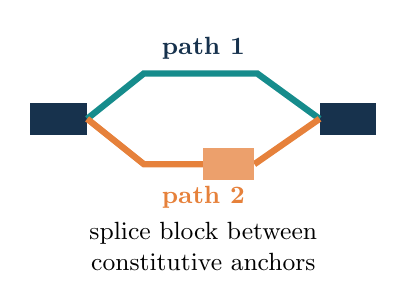
\begin{tikzpicture}[x=0.72cm,y=0.72cm,thick]
\draw[tlGray,line width=2pt] (0,2.2)--(1.0,2.2);
\draw[tlGray,line width=2pt] (5.1,2.2)--(6.1,2.2);
\foreach \x in {0,5.1} \fill[tlNavy] (\x,1.92) rectangle +(1.0,.56);
\draw[tlTeal,line width=2.3pt] (1.0,2.2)--(2.0,3.0)--(4.0,3.0)--(5.1,2.2);
\draw[tlOrange,line width=2.3pt] (1.0,2.2)--(2.0,1.4)--(2.65,1.4)--(3.05,1.4);
\draw[tlOrange,line width=2.3pt] (3.95,1.4)--(5.1,2.2);
\fill[tlOrange!75] (3.05,1.12) rectangle +(0.9,.56);
\node[tlNavy,font=\small\bfseries] at (3.05,3.45) {path 1};
\node[tlOrange,font=\small\bfseries] at (3.05,0.82) {path 2};
\node[align=center,font=\small] at (3.05,-0.05) {splice block between\\constitutive anchors};
\end{tikzpicture}
\end{column}
\begin{column}{0.46\textwidth}
\begin{block}{Two questions}
\small
\textbf{Cell type}, does path usage differ across cell types while condition is unrestricted?

\medskip
\textbf{Condition}, does path usage differ across conditions within one cell type?
\end{block}
\vspace{0.15cm}
\begin{itemize}\scriptsize
\item One hypothesis per nonredundant local path partition
\item Mouse is the biological replication unit
\item Cells contribute to mouse $\times$ condition $\times$ cell-type pseudobulks, never independent replicates
\end{itemize}
\end{column}
\end{columns}
\end{frame}

\begin{frame}{Forward model, splice-path effects $\rightarrow$ isoforms $\rightarrow$ ECs $\rightarrow$ counts}
\centering
\resizebox{\textwidth}{!}{%
\begin{tikzpicture}[node distance=0.55cm,>=Latex,every node/.style={font=\small},box/.style={rounded corners=3pt,draw=tlNavy!55,line width=.7pt,minimum width=2.65cm,minimum height=4.25cm,align=center,inner sep=7pt},arr/.style={->,line width=1.25pt,tlTeal}]
\node[box,fill=tlLightTeal] (path) {\textbf{Local path effects}\\[5pt]$\bm\delta_{bmc}\in\mathbb R^{d_b}$\\$d_b=S_b-1$\\[8pt]\begin{tikzpicture}[x=.3cm,y=.3cm]\draw[tlTeal,line width=1.6pt](0,1)--(1,2)--(3,2)--(4,1);\draw[tlOrange,line width=1.6pt](0,1)--(1,0)--(3,0)--(4,1);\fill[tlNavy](0,.65)rectangle(.7,1.35);\fill[tlNavy](3.3,.65)rectangle(4,1.35);\end{tikzpicture}\\[6pt]perturb pooled\\isoform baseline};
\node[box,fill=tlLight,right=of path] (iso) {\textbf{Isoform composition}\\[5pt]$\bm\eta_{gi,-}\in\mathbb R^{T_g-1}$\\$\bm\theta_{gi}=\operatorname{softmax}\{(\bm\eta_{gi,-}',0)'\}$\\[8pt]
\begin{tikzpicture}[x=.27cm,y=.27cm]\foreach \y/\c in {2/tlTeal,1/tlOrange,0/tlGold}{\draw[\c,line width=1.6pt](0,\y)--(1,\y)--(2,\y+.25)--(3,\y+.25)--(4,\y);\fill[tlNavy](0,\y-.18)rectangle(.7,\y+.18);\fill[tlNavy](3.3,\y-.18)rectangle(4,\y+.18);}\end{tikzpicture}\\shared across primers};
\node[box,fill=tlLight,right=of iso] (ec) {\textbf{EC probabilities}\\[5pt]$A_{gp}\in\mathbb R_+^{K_{gp}\times T_g}$\\[2pt]$\displaystyle\bm q_{gip}=\frac{A_{gp}\bm\theta_{gi}}{\bm1' A_{gp}\bm\theta_{gi}}$\\[8pt]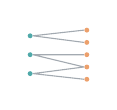
\begin{tikzpicture}[x=.24cm,y=.24cm]\foreach \y in {0,1,2}{\fill[tlTeal!75](0,\y)circle(.13);}\foreach \y in {0,.65,1.3,1.95,2.6}{\fill[tlOrange!75](3,\y-.3)circle(.13);}\draw[tlGray!60](.15,0)--(2.85,-.3) (.15,0)--(2.85,.35) (.15,1)--(2.85,.35) (.15,1)--(2.85,1) (.15,2)--(2.85,1.65) (.15,2)--(2.85,2.3);\end{tikzpicture}\\primer-specific maps};
\node[box,fill=tlLight,right=of ec] (count) {\textbf{Observed counts}\\[5pt]$\bm c_{gip}\in\mathbb N_0^{K_{gp}}$\\[2pt]$\bm c_{gip}\sim\operatorname{Multinomial}(n_{gip},\bm q_{gip})$\\[9pt]
\begin{tikzpicture}[x=.24cm,y=.24cm]\foreach \x/\h/\c in {0/1.0/tlTeal,1/2.2/tlOrange,2/1.5/tlGold,3/2.8/tlTeal,4/.7/tlOrange}{\fill[\c!80](\x,0)rectangle +(0.65,\h);}\end{tikzpicture}\\paired oligo(dT) and\\random-hexamer vectors};
\draw[arr] (path)--(iso);
\draw[arr] (iso)--(ec);
\draw[arr] (ec)--(count);
\end{tikzpicture}
}
\vspace{0.2cm}
\small Ambiguous ECs remain ambiguous, primer design enters through $A_{gp}$, and the same pooled-baseline path perturbation generates both primer observations.
\end{frame}

\begin{frame}{Direct local-path inference uses biological replicates}
\begin{columns}[T,onlytextwidth]
\begin{column}{0.55\textwidth}
\vspace{0.1cm}
\begin{block}{One local fit per mouse and level}
\scriptsize Within-path isoform ratios and nuisance isoforms are fixed at a label-independent pooled baseline. The $d_b=S_b-1$ path coordinates are estimated from both primer-specific EC vectors with two pseudo-observations per path.
\end{block}
\vspace{0.15cm}
\scriptsize For cell types, mouse $m$ contributes the paired path-ILR difference $\widehat{\bm d}_{bm}=\widehat{\bm y}_{bm2}-\widehat{\bm y}_{bm1}\in\mathbb R^{d_b}$.
\vspace{0.2cm}
\begin{itemize}\scriptsize
\item Paired $t$ test for two paths, Hotelling test for more paths
\item Robust variance moderation for scalar tests
\item Multivariate mouse-level regression for condition within cell type
\end{itemize}
\end{column}
\begin{column}{0.42\textwidth}
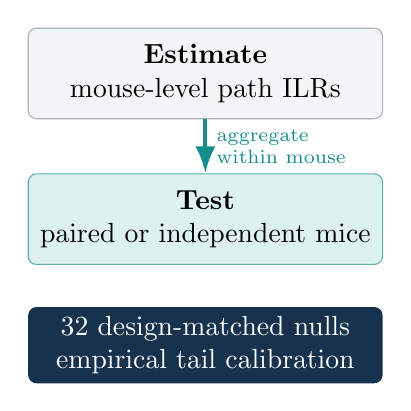
\begin{tikzpicture}[x=1cm,y=1cm,>=Latex]
\node[rounded corners=3pt,fill=tlLight,draw=tlGray!55,minimum width=4.5cm,minimum height=1.15cm,align=center] (estimate) at (0,3.6) {\textbf{Estimate}\\mouse-level path ILRs};
\node[rounded corners=3pt,fill=tlLightTeal,draw=tlTeal!70,minimum width=4.5cm,minimum height=1.15cm,align=center] (test) at (0,1.75) {\textbf{Test}\\paired or independent mice};
\draw[->,tlTeal,line width=1.5pt] (estimate)--node[right,font=\scriptsize,align=left] {aggregate\\within mouse} (test);
\node[rounded corners=3pt,fill=tlNavy,text=white,minimum width=4.5cm,minimum height=.9cm,align=center] at (0,.15) {32 design-matched nulls\\empirical tail calibration};
\end{tikzpicture}
\vspace{0.1cm}
\begin{alertblock}{Calibration matters}
\scriptsize Cell-type labels are sign-flipped within mouse; condition labels are permuted across mice. The complete scoring pipeline is rerun for every null family.
\end{alertblock}
\end{column}
\end{columns}
\end{frame}

\begin{frame}{Two brain datasets, one subject-level analysis design}
\begin{columns}[T,onlytextwidth]
\begin{column}{0.49\textwidth}
\begin{block}{\Large Mouse \hfill \pill{tlTeal}{GSE189033}}
\small
\textbf{Biology}, 5xFAD amyloidosis crossed with Csf1r $\Delta$FIRE microglial deficiency, including PBS and microglia-transplant arms

\medskip
\textbf{Samples}, 48 mice, six groups, balanced 4 female and 4 male per group, age 5--6 months

\medskip
\textbf{Assay}, SPLiT-seq single-nucleus RNA-seq, paired oligo(dT) and random-hexamer observations

\medskip
\textbf{Analysis strata}, 936 mouse $\times$ condition $\times$ cell-type pseudobulks before feature-level support filtering
\end{block}
\end{column}
\begin{column}{0.49\textwidth}
\begin{block}{\Large Human \hfill \pill{tlOrange}{GSE233208}}
\small
\textbf{Biology}, cortical postmortem tissue spanning control, sporadic Alzheimer disease, Down syndrome, and Down syndrome with AD

\medskip
\textbf{Scale}, 396,277 annotated nuclei represented by 40 paired sequencing runs in five batches

\medskip
\textbf{Assay}, Parse Biosciences Evercode WT v1 single-nucleus RNA-seq

\medskip
\textbf{Role}, independent cross-species computational sensitivity for the former global EC GLMM
\end{block}
\end{column}
\end{columns}
\source{Sources, Spangenberg et al., Cell Reports 2022, GEO GSE189033; Miyoshi et al., Nature Genetics 2024, GEO GSE233208. Counts shown are the analysis metadata summarized in this repository.}
\end{frame}

\begin{frame}{Full-data local-path analysis resolves cell-type events}
\begin{columns}[T,onlytextwidth]
\begin{column}{0.49\textwidth}
\centering
\metric{tlTeal}{3,537}{nominal cell-type tests}
\hspace{0.15cm}
\metric{tlOrange}{1,111}{nominal condition tests}
\vspace{0.55cm}
\metric{tlNavy}{2,222}{cell-type BH calls}
\hspace{0.15cm}
\metric{tlGold}{0}{condition BH calls}
\end{column}
\begin{column}{0.48\textwidth}
\vspace{0.05cm}
\begin{itemize}\small
\item 11,315 eligible cell-type-pair tests and 14,833 condition-within-cell-type tests
\item Cell-type calls span 585 blocks and 440 genes
\item Every one of 32 null families has zero BH calls for both contrasts
\item Pooled null rejection is 0.0500, 0.0100, and approximately 0.0010
\end{itemize}
\vspace{0.05cm}
\begin{block}{Interpretation}
\scriptsize The condition family has nominal enrichment but no calibrated BH event. Calibration therefore does not mechanically create a discovery set.
\end{block}
\end{column}
\end{columns}
\end{frame}

\begin{frame}{Direct local-path Tealeaf exceeds junction comparators}
\centering
\scriptsize
\renewcommand{\arraystretch}{1.23}
\setlength{\tabcolsep}{5.5pt}
\begin{tabular}{lrrrrrr}
\toprule
& \multicolumn{3}{c}{Tealeaf} & \multicolumn{3}{c}{Comparator}\\
\cmidrule(lr){2-4}\cmidrule(lr){5-7}
Comparator & Rep. & held & $\rho$ & Rep. & held & $\rho$\\
\midrule
LeafCutter & \textbf{50} & \textbf{0.799} & \textbf{0.711} & 26 & 0.750 & 0.542\\
MAJIQ Heterogen & \textbf{103} & \textbf{0.810} & \textbf{0.622} & 38 & 0.698 & 0.437\\
scQuint & \textbf{101} & \textbf{0.819} & \textbf{0.656} & 56 & 0.775 & 0.458\\
\bottomrule
\end{tabular}
\vspace{0.4cm}
\begin{block}{What the paired local-path test changes}
\scriptsize Subject-level path ILRs are estimated directly from both primer-specific EC vectors, stabilized by add-two smoothing, variance-moderated across scalar tests, and empirically calibrated with 32 sign-flip families. ``Rep.'' applies BH to the conjunction p-value on each pairwise shared gene universe; $\rho$ is fold correlation of gene--pair $-\log_{10}p$.
\end{block}
\begin{alertblock}{Interpretation}
\scriptsize Every aggregated replicated-gene null family has zero BH calls. Add-two smoothing was selected on these splits, so independent-data confirmation remains necessary.
\end{alertblock}
\end{frame}

\begin{frame}{Direct local-path fitting removes the GLMM bottleneck}
\begin{columns}[T,onlytextwidth]
\begin{column}{0.55\textwidth}
\centering
\metric{tlTeal}{2.52 h}{both subject-half fits}
\hspace{0.12cm}
\metric{tlNavy}{1.03 h}{full cell-type fit}
\vspace{0.45cm}
\metric{tlOrange}{0.288 GiB}{peak split worker memory}
\hspace{0.12cm}
\metric{tlGold}{49$\times$}{less worker time\\than former full GLMM}
\end{column}
\begin{column}{0.42\textwidth}
\begin{itemize}\small
\item Raw EC likelihood and both primer maps are retained
\item No latent mouse effect is optimized separately for every hypothesis
\item Each mouse-level composition is fitted once per block and level
\item Condition permutations reuse the label-invariant null REML variance
\end{itemize}
\end{column}
\end{columns}
\source{Worker time starts from prepared inputs and excludes shared read processing. The 49-fold comparison is 51.0 versus 1.03 mouse worker hours.}
\end{frame}

\begin{frame}{Production cell-type blocks include 110 cassette exons}
\begin{columns}[T,onlytextwidth]
\begin{column}{0.52\textwidth}
\resizebox{\linewidth}{!}{%
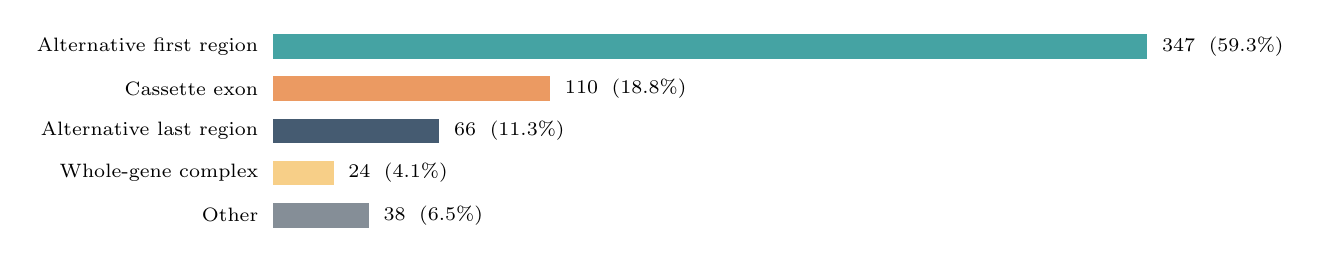
\begin{tikzpicture}[x=.032cm,y=.63cm]
\foreach \i/\name/\v/\pct/\clr in {0/Alternative first region/347/59.3/tlTeal,1/Cassette exon/110/18.8/tlOrange,2/Alternative last region/66/11.3/tlNavy,3/Whole-gene complex/24/4.1/tlGold,4/Other/38/6.5/tlGray}{\node[anchor=east,font=\scriptsize] at (-2,4.6-\i*.85) {\name};\fill[\clr!80] (0,4.35-\i*.85) rectangle (\v,4.85-\i*.85);\node[anchor=west,font=\scriptsize] at (\v+2,4.6-\i*.85) {\v\; (\pct\%)};}
\end{tikzpicture}
}
\end{column}
\begin{column}{0.45\textwidth}
\small
\textbf{Functional precedents among production calls}
\vspace{0.15cm}
\begin{itemize}\scriptsize
\item \textit{Ntrk2}, alternative last region separating short kinase-deficient and long TrkB paths; TrkB.T1 has a characterized astrocyte role
\item \textit{Grin1}, C1 cassette exon linked to receptor surface trafficking
\item \textit{App}, exon 15 cassette linked to polarized secretion and amyloid processing
\item \textit{Dlg4}, alternative-first-region block overlapping functional PSD-95 alpha/beta starts
\end{itemize}
\vspace{0.05cm}
\begin{alertblock}{Boundary of the annotation}
\scriptsize A terminal-region label means supported paths differ between a constitutive anchor and a transcript boundary. It does not by itself distinguish promoter choice, terminal exon choice, or polyadenylation.
\end{alertblock}
\end{column}
\end{columns}
\end{frame}

\begin{frame}{Takeaways}
\vspace{0.1cm}
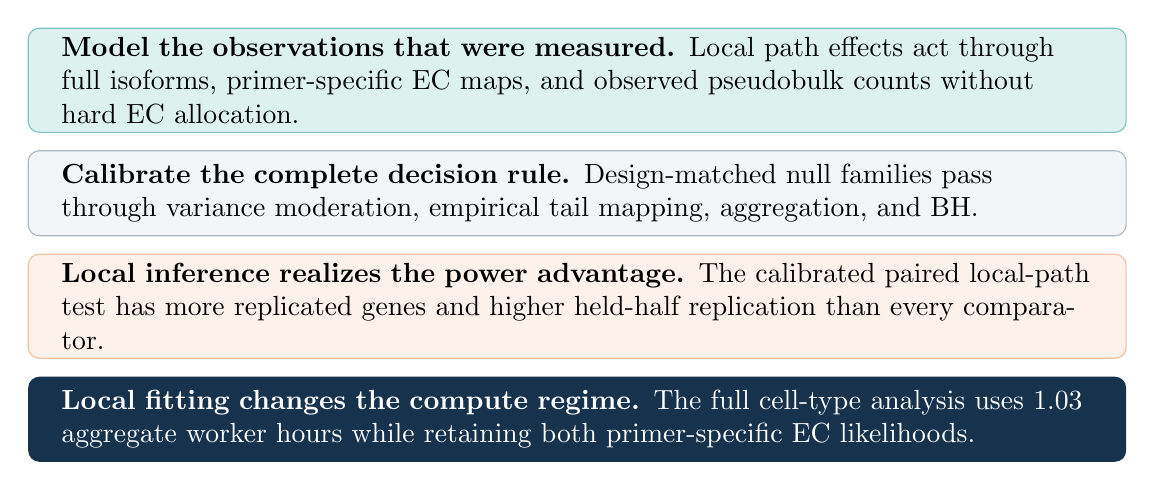
\begin{tikzpicture}[node distance=.22cm,box/.style={rounded corners=4pt,minimum width=13.9cm,minimum height=1.08cm,text width=13.1cm,align=left,inner xsep=12pt,font=\normalsize}]
\node[box,fill=tlLightTeal,draw=tlTeal!55] (a) {\textbf{Model the observations that were measured.} Local path effects act through full isoforms, primer-specific EC maps, and observed pseudobulk counts without hard EC allocation.};
\node[box,fill=tlLight,draw=tlNavy!35,below=of a] (b) {\textbf{Calibrate the complete decision rule.} Design-matched null families pass through variance moderation, empirical tail mapping, aggregation, and BH.};
\node[box,fill=tlOrange!10,draw=tlOrange!50,below=of b] (c) {\textbf{Local inference realizes the power advantage.} The calibrated paired local-path test has more replicated genes and higher held-half replication than every comparator.};
\node[box,fill=tlNavy,text=white,below=of c] (d) {\textbf{Local fitting changes the compute regime.} The full cell-type analysis uses 1.03 aggregate worker hours while retaining both primer-specific EC likelihoods.};
\end{tikzpicture}
\end{frame}

\end{document}
